%%%%%%%%%%%%%%%%%%%%%%%%%%%%%%%%%%%%%%%%%
% FRI Data Science_report LaTeX Template
% Version 1.0 (28/1/2020)
% 
% Jure Demšar (jure.demsar@fri.uni-lj.si)
%
% Based on MicromouseSymp article template by:
% Mathias Legrand (legrand.mathias@gmail.com) 
% With extensive modifications by:
% Antonio Valente (antonio.luis.valente@gmail.com)
%
% License:
% CC BY-NC-SA 3.0 (http://creativecommons.org/licenses/by-nc-sa/3.0/)
%
%%%%%%%%%%%%%%%%%%%%%%%%%%%%%%%%%%%%%%%%%


%----------------------------------------------------------------------------------------
%	PACKAGES AND OTHER DOCUMENT CONFIGURATIONS
%----------------------------------------------------------------------------------------
\documentclass[fleqn,moreauthors,10pt]{ds_report}
\usepackage[english]{babel}

\graphicspath{{fig/}}




%----------------------------------------------------------------------------------------
%	ARTICLE INFORMATION
%----------------------------------------------------------------------------------------

% Header
\JournalInfo{FRI Natural language processing course 2025}

% Interim or final report
\Archive{Project report} 
%\Archive{Final report} 

% Article title
\PaperTitle{Conversational Agent with Retrieval-Augmented Generation for research assistance} 

% Authors (student competitors) and their info
\Authors{Marko Medved, Sebastijan Trojer, and Matej Vrečar}

% Advisors
\affiliation{\textit{Advisors: Aleš Žagar}}

% Keywords
\Keywords{Retrieval augmented generation, research assistance, re-identification}
\newcommand{\keywordname}{Keywords}


%----------------------------------------------------------------------------------------
%	ABSTRACT
%----------------------------------------------------------------------------------------

\Abstract{
Large language models (LLMs) are increasingly used in conversational agents for academic support, but they often struggle with outdated knowledge and hallucinations in specialized domains. To address this, we developed a conversational assistant using Retrieval-Augmented Generation (RAG), focusing on the field of automatic re-identification. Our system retrieves recent research papers from arXiv and CVF, processes them using domain-adapted query rewriting and relevance-based re-ranking, and integrates this context into language model responses. We implemented and evaluated both a baseline and an improved retrieval pipeline, emphasizing relevance over exact matches. 
% TODO results
}

%----------------------------------------------------------------------------------------

\begin{document}

% Makes all text pages the same height
\flushbottom 

% Print the title and abstract box
\maketitle 

% Removes page numbering from the first page
\thispagestyle{empty} 

%----------------------------------------------------------------------------------------
%	ARTICLE CONTENTS
%----------------------------------------------------------------------------------------

\section*{Introduction}
We are developing a conversational agent with Retrieval-Augmented 
Generation (RAG) to support academic research, focusing on the field of automatic
 re-identification. The system will leverage a pre-trained chatbot developed in
  [TODO insert year], enhanced with a RAG mechanism to retrieve and incorporate the 
  latest research papers from arXiv. To keep the model manageable and focused, 
  we will limit the scope of retrieved papers to a specific recent time frame 
  (e.g., one month). The retrieved papers will be processed and integrated into 
  the chatbot's responses, allowing the agent to provide up-to-date and accurate 
  answers about re-identification methods developed after the chatbot’s original 
  training. To evaluate our approach an option is to manually check if the answers
   were relevant for the chosen scientific area and if the papers used for the
    queries were relevant for the specific query. Another option would be to compare
     the answers of a chat-bot that was trained with more recent data. Possible 
     pre-trained chatbots that we could use include Mistral 7B or Zephyr. 





%------------------------------------------------

\section*{Related work}

% Joined

Large Language Models (LLMs) have demonstrated strong language understanding and generation capabilities, but they often struggle with hallucinations, outdated knowledge, and limited domain-specific accuracy, especially when handling specialized research queries~\cite{kandpal2023longtail}. Retrieval-Augmented Generation (RAG) addresses these challenges by enhancing LLMs with real-time information retrieval, improving factual accuracy and relevance~\cite{gao2024rag}. Early RAG models followed a basic retrieve-then-generate structure, but more advanced approaches have introduced techniques like query rewriting, reranking, and adaptive retrieval to improve context relevance and coherence~\cite{gao2024rag}.

Recent research has shown the effectiveness of RAG-based systems for academic and domain-specific applications. For example,~\cite{Chatbots_in_Academia} implemented a RAG system using OpenAI Ada embeddings and GPT-3.5 to enhance information retrieval and synthesis for academic documents, demonstrating the importance of precise embedding strategies for research-based chatbots. Afzal et al.~\cite{afzal2024towards} focused on domain-specific data by creating the CurriculumQA dataset and optimizing retrieval with tailored evaluation metrics such as relevance, coherence, and faithfulness, highlighting the importance of fine-tuning for specific academic fields. Similarly, Yasin et al.~\cite{yasin2024retrieval} integrated advanced techniques—including fine-tuned embedding models, semantic chunking, and abstract-first retrieval—to improve the accuracy and relevance of scholarly content retrieval.

Evaluating RAG systems remains complex due to the nuanced nature of retrieval and generation quality. Chen et al.~\cite{chen2024benchmarking} introduced the Retrieval-Augmented Generation Benchmark (RGB) to measure RAG performance across four key dimensions: noise robustness, negative rejection, information integration, and counterfactual robustness. Their findings show that while RAG improves LLM accuracy, it still struggles with integrating long-distance information and handling noisy or uncertain evidence. Common evaluation methods for RAG systems include retrieval-focused metrics like MRR (Mean Reciprocal Rank) and nDCG (normalized Discounted Cumulative Gain), as well as generation-focused metrics like BLEU and ROUGE to measure the quality and relevance of generated responses~\cite{lewis2020rag}.

In our project, we aim to address these issues by developing a RAG-based chatbot for academic research in automatic re-identification—the task of matching individuals across different cameras or settings, a complex problem in computer vision and machine learning. By focusing on recent research papers from arXiv, we seek to enhance the chatbot’s ability to retrieve and generate accurate responses about the latest developments in automatic re-identification


\section*{Methods}
\subsection*{Baseline}
\subsubsection*{Paper Retrieval from arXiv}
We begin by retrieving candidate papers using the official arXiv API. For each paper, we extract its title, abstract, and metadata. To enable semantic similarity-based filtering, both the user query and the abstracts are embedded using the \texttt{allenai-specter} SentenceTransformer model, which is trained to map scientific documents into a dense vector space. We compute cosine similarity between the query embedding and each abstract embedding, and select the top-$k$ most relevant papers ($k=30$ by default).

\subsubsection*{Context Construction}
The titles and abstracts of the top-ranked papers are concatenated into a single text block to serve as external context. This context is inserted into the prompt presented to the language model. No chunking, reranking, or content selection is applied at this stage beyond the similarity-based retrieval.

\subsubsection*{Language Model Inference}
We use \texttt{Mistral-7B-Instruct-v0.2} as the language model backend. To enable efficient inference on commodity hardware, the model is loaded using 4-bit quantization with \texttt{bitsandbytes}, applying NF4 quantization and bfloat16 compute precision. The model is wrapped with Hugging Face's text-generation pipeline and integrated with LangChain to enable prompt-based question answering. Prompt templates include both the constructed context and the current user query. For comparison, we also evaluate answers generated without any retrieved context.

\subsubsection*{System Behavior}
The system retains a basic conversational memory by concatenating the most recent user query with the current one. This helps preserve short-term context without implementing a full dialogue memory or rewriting mechanism. No fine-tuning is performed, and no re-ranking, filtering, or external knowledge base is used. This baseline is intended to evaluate performance with minimal architectural complexity.


  \subsection*{Improved model}

Several enhancements were implemented over the baseline RAG system to 
improve relevance and accuracy, particularly for person re-identification
 from video:

\begin{itemize}
    \item \textbf{Two-Stage Query Rewriting}: Queries are rewritten separately for retrieval (search) and semantic matching, improving both recall and ranking quality.
    
    \item \textbf{Domain-Specific Augmentation}: Rewritten queries are enriched with terms like \texttt{"person re-identification"} and restricted to the \texttt{cs.CV} category to focus results on relevant literature.

    \item \textbf{Local Database Integration}: Retrieval includes a local CVF paper database, expanding coverage beyond arXiv.

    \item \textbf{Unified Re-Ranking}: All retrieved papers are encoded with \texttt{allenai-specter} and re-ranked using cosine similarity against the rewritten match query.

    \item \textbf{Task-Specific Prompting}: The LLM prompt is tailored for the Re-ID task, improving the domain alignment of generated responses.
\end{itemize}

Figure~\ref{fig:retrieval_pipeline} illustrates the improved retrieval pipeline, highlighting the two-stage query rewriting, local CVF integration, and re-ranking stages.


\begin{figure}[h]
    \centering
    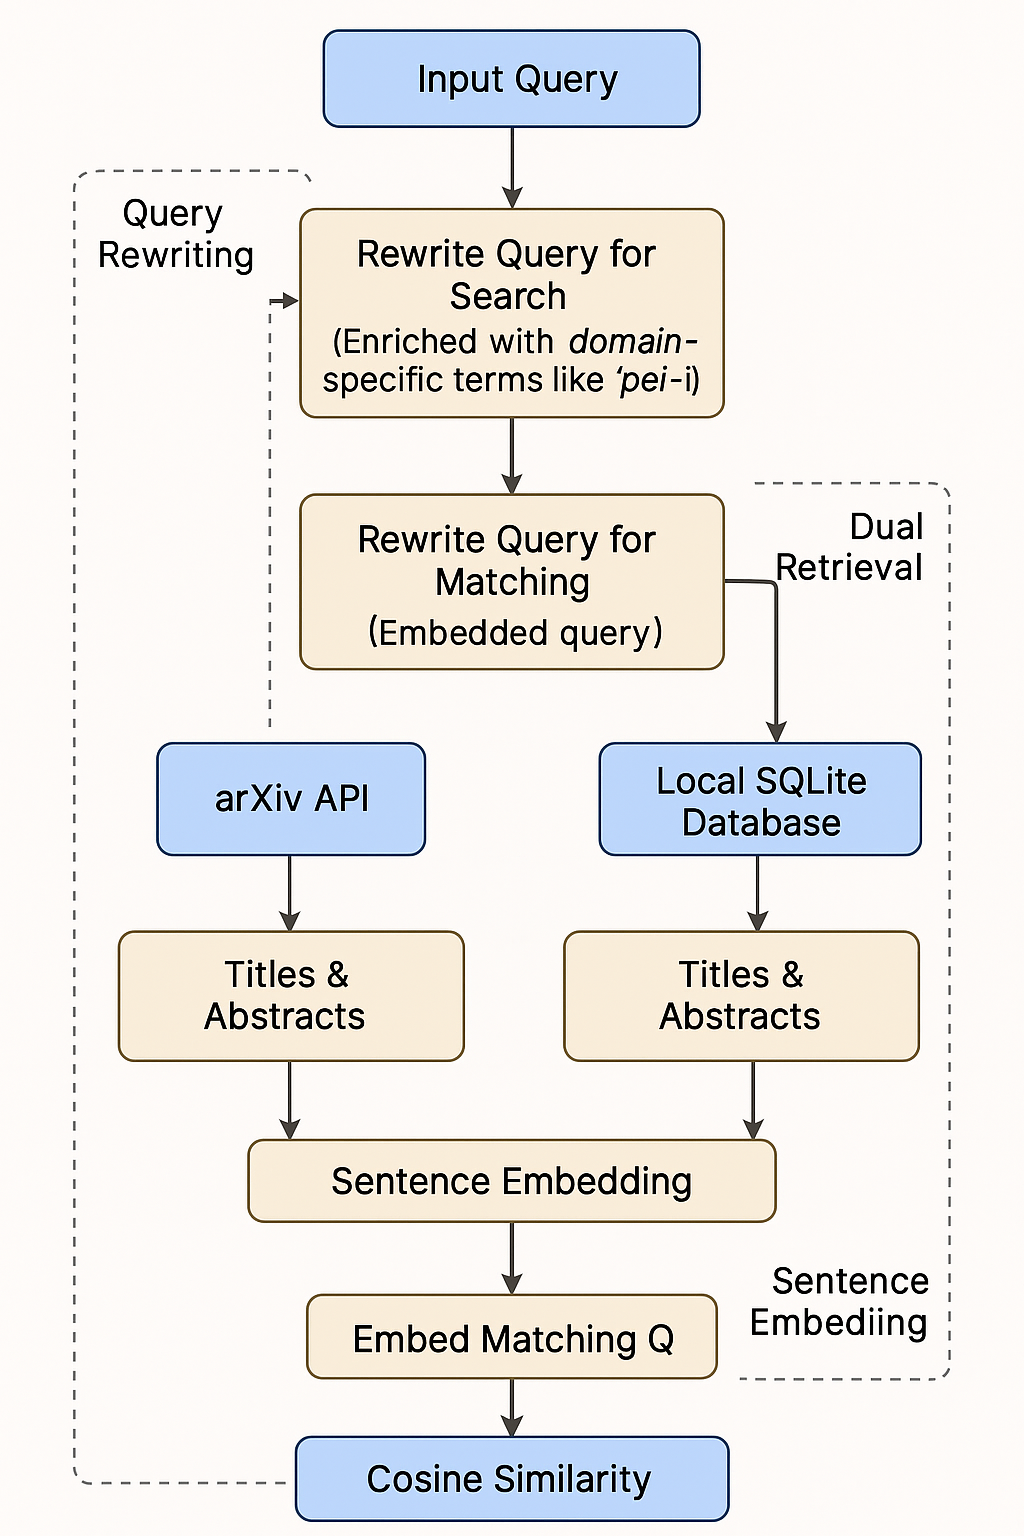
\includegraphics[width=\linewidth]{fig/tmp.png}
    \caption{Tmp flowchart}
    \label{fig:retrieval_pipeline}
\end{figure}





\section*{Results}
\subsection*{Preliminary results }
To evaluate the effectiveness of our RAG-enhanced approach, we tested it on scientific
 questions related to papers published after December 2023. The goal was to determine 
 whether the system could incorporate recent research not seen during the original
  model’s training.

Across a range of prompts, results showed that while the system often failed to retrieve 
the exact target paper with top-$k=5$, it still produced more informative and current responses by leveraging similar recent articles. Increasing $k$ to 10 improved retrieval in several cases—for example, retrieving a nearly identical sentiment analysis paper by the same authors.

Refined queries also led to improved results. For a fast and robust covariance estimator, adding terms like “low contamination regime” and “near-linear sample complexity” helped surface the correct article. In contrast, generic queries often led the model to irrelevant domains, such as quantum mechanics.

For topics like NP-complete problems and object detection, specificity again proved critical. While exact matches were rare, the RAG system offered responses more reflective of recent research trends than the baseline. However, it occasionally exhibited erratic behavior, such as generating its own sub-questions, which significantly increased inference time.

Overall, these preliminary findings, detailed further in \texttt{results/testing\_the\_model.docx},
 suggest that RAG enhances response relevance and currency, particularly with higher $k$
  and well-formed queries. However, retrieval control and relevance filtering remain
  areas for future improvement. Note that these results were collected using the baseline method. 
  
\subsection*{Final Results}
Since we mostly focused on improving the retrieval side of our model, here we use a 
metric similar to the CMC - a metric often used in computer vision recognition tasks. 



%------------------------------------------------


%------------------------------------------------

\section*{Discussion}

Use the Discussion section to objectively evaluate your work, do not just put praise on everything you did, be critical and exposes flaws and weaknesses of your solution. You can also explain what you would do differently if you would be able to start again and what upgrades could be done on the project in the future.


%----------------------------------------------------------------------------------------
%	REFERENCE LIST
%----------------------------------------------------------------------------------------
\bibliographystyle{unsrt}
\bibliography{report}


\end{document}
